% ---------------------------------------------------------------------------
% Thai version of story_template.tex, laid out after the KMITL Thai short-paper
% template ([THAI]Templete_Short Paper.pdf): A4, TH Sarabun, page 1 in one
% column (title, abstract, keywords, author footnotes), body in two columns,
% Thai section headings, "ตารางที่/รูปที่" captions and numbered APA-style
% references. Every number is copied from story_template.tex; if a number
% changes there, change it here too.
% Build (XeTeX is required for Thai): cd paper && tectonic story_template_th.tex
% Font: TH Sarabun New or TH SarabunPSK if installed (as in the template),
% otherwise Sarabun.
% ---------------------------------------------------------------------------
\documentclass[11pt,a4paper]{article}
\usepackage[a4paper,top=2.5cm,bottom=2.5cm,left=2.5cm,right=2.5cm,columnsep=0.8cm]{geometry}
\usepackage{amsmath}
\usepackage{fontspec}
\IfFontExistsTF{TH Sarabun New}{%
  \setmainfont{TH Sarabun New}[Scale=1.45]\linespread{1.05}}{%
  \IfFontExistsTF{TH SarabunPSK}{%
    \setmainfont{TH SarabunPSK}[Scale=1.45]\linespread{1.05}}{%
    \setmainfont{Sarabun}\linespread{1.2}}}
\XeTeXlinebreaklocale "th"
% Stretch at Thai word boundaries, so justification spreads over many small
% gaps instead of a few wide ones (PDF review, round 2).
\XeTeXlinebreakskip = 0pt plus 1.5pt
\usepackage{graphicx}
\graphicspath{{../}}
\usepackage{array}
\usepackage{xcolor}
\usepackage[hyphens]{url}
\usepackage{enumitem}
\usepackage{titlesec}
\usepackage{caption}

\newif\ifshowtodos
\showtodostrue
\newcommand{\todo}[1]{\ifshowtodos\textcolor{red}{[TODO: #1]}\fi}

\pagestyle{empty}
\setlength{\parindent}{1cm}
\setlength{\emergencystretch}{4em}
% Keep line spacing uniform: stacked Thai vowels and tone marks would
% otherwise push some lines apart.
\setlength{\lineskiplimit}{-\maxdimen}
% Do not start or end a paragraph with a single line at a column break.
\clubpenalty=10000
\widowpenalty=10000
\newcolumntype{L}[1]{>{\raggedright\arraybackslash}p{#1}}

% Headings as in the template: "1. บทนำ", "1.1 ...", "3.1.1 ..." (indented).
\titleformat{\section}{\normalfont\large\bfseries\raggedright}{\thesection.}{0.4em}{}
\titlespacing*{\section}{0pt}{1.1em}{0.4em}
\titleformat{\subsection}{\normalfont\normalsize\bfseries\raggedright}{\thesubsection}{0.5em}{}
\titlespacing*{\subsection}{0pt}{0.6em}{0.2em}
\titleformat{\subsubsection}{\normalfont\normalsize\bfseries\raggedright}{\thesubsubsection}{0.5em}{}
\titlespacing*{\subsubsection}{1cm}{0.4em}{0.1em}

% Captions as in the template: italic, "ตารางที่ 1 ..." above tables and
% "รูปที่ 1 ..." below figures.
\renewcommand{\figurename}{รูปที่}
\renewcommand{\tablename}{ตารางที่}
\captionsetup{font={small,it},labelfont={small,it},labelsep=space}
\captionsetup[table]{position=top,justification=raggedright,singlelinecheck=false}

% Run-in labels for the four-part story of each case.
\newcommand{\storylabel}[1]{\textbf{#1}\quad}

\begin{document}

% ===========================================================================
% Page 1: one column, as in the template
% ===========================================================================
\begin{center}
{\Large\bfseries ผ่านการตรวจแล้ว แต่ผิด (Validated, yet Wrong):\\[0.2em]
บทเรียนจากการทบทวนการตรวจสอบความถูกต้อง\\[0.2em]
ของงานเมแทบอโลมิกส์สี่กรณี\par}
\vspace{1.2em}
{\bfseries คณิณ แคลวิณ ชมวิวัฒน์\textsuperscript{*1} และ ชัยพร ออฤดี\textsuperscript{1}\par}
\vspace{0.6em}
{\bfseries คณะเทคโนโลยีสารสนเทศ สถาบันเทคโนโลยีพระจอมเกล้าเจ้าคุณทหารลาดกระบัง\par}
\vspace{0.4em}
{\bfseries เลขที่ 1 ซอยฉลองกรุง 1 แขวงลาดกระบัง เขตลาดกระบัง กรุงเทพฯ 10520\par}
\end{center}

\vspace{1.5em}
\noindent\textbf{บทคัดย่อ}

การศึกษานี้ทบทวนงานวิเคราะห์ด้วยการเรียนรู้ของเครื่อง (Machine Learning)
สี่งานของผู้วิจัยเอง ซึ่งใช้ข้อมูลเมแทบอโลมิกส์ (Metabolomics) จาก NMR
ขนาดเล็กที่เผยแพร่สาธารณะ แต่ละงานให้ผลที่ผู้วิจัยเคยถือว่าผ่านการตรวจสอบความถูกต้องแล้ว
ได้แก่ ค่า \textit{p} จากการทดสอบเรียงสับเปลี่ยน (Permutation Test)
ที่ต่ำที่สุดเท่าที่การทดสอบจะให้ได้ เส้นโค้ง ROAR ที่ต่ำกว่าการตัดฟีเจอร์แบบสุ่ม
หรือคะแนนสูงจากการตรวจสอบไขว้ (Cross-Validation) ที่แบ่งกลุ่มตามบุคคล
แต่ในทั้งสี่งาน การตีความทางชีววิทยาที่ผู้วิจัยให้กับคะแนนนั้นไม่มีหลักฐานรองรับ
หรือไม่สามารถระบุได้
แบบจำลองพยากรณ์ผู้ตอบสนองต่อการผ่าตัดที่ได้ค่า \textit{p} = 0.001
จากวิธีที่ยังไม่ได้ตรวจการสอบเทียบ (Calibration)
ทำได้ไม่ดีไปกว่าคะแนนอ้างอิงที่ไม่ต้องฝึกแบบจำลอง และความเชื่อมโยงระหว่างผลลัพธ์ที่คำนวณจากการเปลี่ยนแปลงกับฟีเจอร์ค่าตั้งต้น
สามารถอธิบายสมรรถนะของแบบจำลองได้โดยไม่ต้องมีการตอบสนองที่พยากรณ์ได้
สารสามชนิดที่ยังไม่ทราบแหล่งที่มาแน่ชัดถูกจัดอันดับใกล้เคียงกับเมแทบอไลต์ที่เป็นที่ยอมรับในการเปรียบเทียบ
ROAR เชิงสำรวจ ซึ่งไม่สามารถตัดสินแหล่งที่มาของฟีเจอร์ได้
สำหรับตัวจำแนกโรคเบาหวาน ข้อมูลไม่สามารถแยกได้ว่าสมรรถนะเกิดจากความแตกต่างของโรค
หรือจากโปรโตคอลการเก็บตัวอย่างสองแบบที่แต่ละคลาสมาจาก และตัวจำแนก ``โรคอ้วน'' แท้จริงแล้วเปรียบเทียบผู้ป่วยก่อนและหลังการผ่าตัดลดน้ำหนัก
ในข้อมูลจำลองที่ไม่มีการตอบสนองที่พยากรณ์ได้และความเที่ยงของการวัดต่ำ
การทดสอบเรียงสับเปลี่ยนแบบสลับป้ายกำกับทั้งชุดปฏิเสธสมมติฐานความเป็นอิสระในร้อยละ 26
ของชุดข้อมูลเมื่อ \textit{n} = 50 และร้อยละ 100 เมื่อ \textit{n} = 500
ผู้วิจัยเสนอว่ารายงานการตรวจสอบความถูกต้องควรระบุคำอธิบายทางเลือกของคะแนนหลัก
และระบุว่าการทดสอบใดใช้ตรวจคำอธิบายแต่ละข้อ
พร้อมเสนอคำถามหกข้อสำหรับงานเมแทบอโลมิกส์ที่มีขนาดตัวอย่างเล็ก

\vspace{1em}
\noindent\textbf{คำสำคัญ:} การตรวจสอบความถูกต้อง, เมแทบอโลมิกส์, การเรียนรู้ของเครื่อง,
การทดสอบเรียงสับเปลี่ยน, การถดถอยเข้าหาค่าเฉลี่ย, การอธิบายฟีเจอร์, ตัวแปรกวน

\vfill
\noindent\makebox[\linewidth]{\leaders\hbox to 0.45em{\hss-\hss}\hfill}\par
{\small
\noindent * Author's Email: 67070015@kmitl.ac.th\par
\noindent\textsuperscript{1} นักศึกษา คณะเทคโนโลยีสารสนเทศ
สถาบันเทคโนโลยีพระจอมเกล้าเจ้าคุณทหารลาดกระบัง\par}

% ===========================================================================
% Body: two columns from page 2
% ===========================================================================
\twocolumn

\section{บทนำ}
\label{sec:intro}

\subsection{ที่มาและความสำคัญ}

ผลการวิเคราะห์แรกที่ผู้วิจัยนำมาทบทวนเป็นผลที่ผู้วิจัยเคยพอใจมาก
ผู้วิจัยต้องการพยากรณ์จากตัวอย่างเลือดก่อนผ่าตัดเพียงครั้งเดียวว่า
ผู้ป่วยผ่าตัดลดน้ำหนัก (Bariatric Surgery) คนใดจะเป็น ``ผู้ตอบสนองดี''
(Strong Responder) เมื่อครบหนึ่งปี แบบจำลองได้ค่า PR-AUC 0.683
เทียบกับความชุก (Prevalence) 0.437 ผู้วิจัยทำการตรวจสอบไขว้ทั้งหมดซ้ำ
1,000 ครั้ง โดยสลับป้ายกำกับ (Label) ของข้อมูลฝึกภายในแต่ละ Fold
และฝึกแบบจำลองใหม่ทุกครั้ง ไม่มีรอบใดที่ได้ผลดีเท่าแบบจำลองจริง จึงได้ค่า
\textit{p} = 0.001 ซึ่งเป็นค่าต่ำที่สุดที่การสลับ 1,000 รอบจะให้ได้
ตามเกณฑ์การตรวจสอบที่ผู้วิจัยรู้จัก ผลนี้จึงดูเหมือนผ่านการตรวจสอบความถูกต้องแล้ว

ต่อมาผู้วิจัยเปรียบเทียบกับคะแนนอ้างอิงที่ไม่ต้องฝึกแบบจำลอง (Learn-Nothing Scorer)
ซึ่งคำนวณด้วยกฎตายตัวจากค่าตั้งต้น (Baseline) ของผู้ป่วยแต่ละคนและทิศทางที่คาดหวังของสารบ่งชี้แต่ละตัวเท่านั้น
คะแนนนี้ได้ 0.709 สูงกว่าแบบจำลองที่ฝึกแล้ว
ผลการทดสอบเรียงสับเปลี่ยนเป็นเพียงสิ่งบ่งชี้ว่าฟีเจอร์กับป้ายกำกับมีความสัมพันธ์กัน
แต่ไม่สามารถบอกได้ว่าความสัมพันธ์นั้นมาจากอะไร
ป้ายกำกับถูกสร้างจากการเปลี่ยนแปลงระหว่างค่าตั้งต้นกับค่าติดตามผลของผู้ป่วยแต่ละคน
และการสร้างป้ายกำกับในลักษณะนี้อาจทำให้ป้ายกำกับขึ้นกับค่าตั้งต้น
ผ่านความคลาดเคลื่อนของการวัดและการถดถอยเข้าหาค่าเฉลี่ย (Regression to the Mean)
ความเชื่อมโยงนี้สามารถอธิบายสมรรถนะของแบบจำลองได้โดยไม่ต้องมีการตอบสนองทางชีววิทยาที่พยากรณ์ได้
และแบบจำลองที่ฝึกแล้วก็ไม่ได้ดีกว่าคะแนนอ้างอิงนี้

บทความนี้ว่าด้วยระยะห่างระหว่างการตรวจสอบที่ผ่านกับการตีความที่ถูกต้อง
ผู้วิจัยทบทวนงานวิเคราะห์ข้อมูลสาธารณะสี่งานของตนเอง
ซึ่งแต่ละงานดูเหมือนผ่านการตรวจสอบที่ผู้วิจัยใช้
และพบว่าในทั้งสี่งาน การตีความคะแนนของผู้วิจัยไม่มีหลักฐานรองรับ
รายละเอียดเชิงเทคนิคและการศึกษาด้วยการจำลองฉบับเต็มอยู่ในบทความคู่กัน \cite{vyw}
ในบทความนี้ ผู้วิจัยนำเสนอทั้งสี่กรณีในฐานะข้อผิดพลาดที่เกิดขึ้นจริง
เพราะการเข้าใจว่าข้อผิดพลาดรอดผ่านการตรวจสอบได้อย่างไร
มีประโยชน์ต่อนักวิเคราะห์คนถัดไปมากกว่าวิธีแก้ไขเพียงอย่างเดียว
ข้อกล่าวอ้างของบทความนี้มีขอบเขตแคบ
ผู้วิจัยไม่ได้ประเมินว่าความล้มเหลวลักษณะนี้พบบ่อยเพียงใดในงานวิจัยที่ตีพิมพ์
แต่แสดงให้เห็นว่าความล้มเหลวนี้เกิดขึ้นได้ในงานที่ทำอย่างระมัดระวัง
และการตรวจสอบเองก็ไม่ได้ส่งสัญญาณเตือนใด ๆ

\subsection{วัตถุประสงค์ของการศึกษา}
\begin{enumerate}[label=1.2.\arabic*, leftmargin=*, labelindent=0.4cm]
  \item เพื่อทบทวนงานวิเคราะห์ด้วยการเรียนรู้ของเครื่องสี่งานของผู้วิจัย
        ที่ผ่านการตรวจสอบมาตรฐาน แต่การตีความทางชีววิทยาไม่มีหลักฐานรองรับ
  \item เพื่อระบุว่าการตรวจสอบแต่ละแบบตอบคำถามใด และยังเปิดช่องให้คำอธิบายทางเลือกใด
        พร้อมเสนอวิธีควบคุมที่ตรงจุด
  \item เพื่อเสนอแนวคำถามสำหรับการรายงานผลการตรวจสอบความถูกต้อง
        ในงานเมแทบอโลมิกส์ที่มีขนาดตัวอย่างเล็ก
\end{enumerate}

\subsection{ประโยชน์ที่คาดว่าจะได้รับ}
\begin{enumerate}[label=1.3.\arabic*, leftmargin=*, labelindent=0.4cm]
  \item ได้ตัวอย่างจริงของกรณีที่การตรวจสอบมาตรฐานผ่าน แต่การตีความผลไม่ถูกต้อง
        พร้อมวิธีควบคุมที่ใช้ตรวจจับ
  \item ได้แนวคำถามที่นักวิเคราะห์สามารถนำไปใช้ก่อนรายงานคะแนนหลักของแบบจำลอง
\end{enumerate}

% ===========================================================================
\section{ทฤษฎีและงานวิจัยที่เกี่ยวข้อง}
\label{sec:lit}

การตรวจสอบสามแบบที่ผู้วิจัยใช้ทำหน้าที่ต่างกัน
แต่ละแบบตรวจรูปแบบความล้มเหลวเฉพาะอย่างภายใต้สมมติฐานที่กำหนด
และไม่มีแบบใดยืนยันการตีความทางชีววิทยาได้ทั้งหมด
ตารางที่~\ref{tab:gap} แสดงคำถามที่การตรวจสอบแต่ละแบบตอบ
คำถามที่มักถูกเข้าใจว่าตอบ
และคำอธิบายทางเลือกที่การตรวจสอบนั้นยังเปิดช่องไว้ในกรณีของผู้วิจัย

\begin{table*}[t]
\caption{คำถามที่การตรวจสอบแต่ละแบบตอบ คำถามที่มักถูกเข้าใจว่าตอบ
และคำอธิบายทางเลือกที่ยังเปิดอยู่ในกรณีของผู้วิจัย}
\label{tab:gap}
\centering
\small
\begin{tabular}{|L{2.3cm}|L{3.1cm}|L{3.1cm}|L{4.2cm}|c|}
\hline
\textbf{การตรวจสอบ} & \textbf{คำถามที่ตอบ} & \textbf{คำถามที่มักถูกเข้าใจว่าตอบ} & \textbf{คำอธิบายทางเลือกที่ยังเปิดอยู่} & \textbf{กรณี} \\
\hline
Label Permutation & ฟีเจอร์กับป้ายกำกับเป็นอิสระต่อกันหรือไม่ & แบบจำลองพยากรณ์การตอบสนองรายบุคคลได้จริงหรือไม่ & ป้ายกำกับที่คำนวณจากการเปลี่ยนแปลงขึ้นกับฟีเจอร์ค่าตั้งต้นผ่านการถดถอยเข้าหาค่าเฉลี่ย & 1 \\
\hline
ROAR & แบบจำลองพึ่งพาฟีเจอร์อันดับต้นหรือไม่ & ฟีเจอร์อันดับต้นเป็นสัญญาณทางชีววิทยาหรือไม่ & ฟีเจอร์อันดับต้นอาจสะท้อนการจัดการตัวอย่าง ร่วมกับหรือแทนสรีรวิทยา & 2 \\
\hline
Subject-Grouped CV & แบบจำลองพยากรณ์บุคคลใหม่ที่เก็บตัวอย่างด้วยวิธีเดียวกันได้ดีเพียงใด & คะแนนสะท้อนโรคหรือไม่ & แต่ละคลาสเก็บตัวอย่างภายใต้โปรโตคอลของตนเอง & 3 \\
\hline
Subject-Grouped CV & เช่นเดียวกับข้างต้น & ป้ายกำกับมีความหมายตรงกับชื่อหรือไม่ & ป้ายกำกับแทนการเปรียบเทียบอื่น & 4 \\
\hline
\end{tabular}
\end{table*}

\subsection{การตรวจสอบไขว้ (Cross-Validation)}
การตรวจสอบไขว้ไม่ใช่การทดสอบสมมติฐาน
แต่เป็นการประมาณว่าแบบจำลองพยากรณ์ตัวอย่างที่ไม่ได้ใช้ฝึกได้ดีเพียงใด
โดยตัวอย่างเหล่านั้นต้อง\textit{เก็บด้วยวิธีเดียวกัน}กับตัวอย่างที่ใช้ฝึก
การแบ่ง Fold ตามบุคคล (Subject-Grouped) ช่วยตรวจคำอธิบายทางเลือกหนึ่งข้อ
คือแบบจำลองจำบุคคลได้แทนที่จะแยกคลาส
หากตัวอย่างทุกตัวของคลาสหนึ่งถูกเก็บด้วยวิธีที่ต่างจากอีกคลาส
การตรวจสอบไขว้ก็จะรายงานได้อย่างถูกต้องว่าความแตกต่างนั้นใช้ได้กับข้อมูลใหม่

\subsection{การทดสอบเรียงสับเปลี่ยนป้ายกำกับ (Label Permutation Test)}
การทดสอบเรียงสับเปลี่ยนป้ายกำกับทดสอบสมมติฐานว่างที่ว่าฟีเจอร์กับป้ายกำกับเป็นอิสระต่อกัน
\cite{ojala2010} ภายใต้สมมติฐานของการทดสอบ ค่า \textit{p} ที่ต่ำเป็นหลักฐานว่ามีความสัมพันธ์\textit{บางอย่าง}
แต่ไม่ได้บอกว่าความสัมพันธ์นั้นมาจากไหน การสลับป้ายกำกับทำได้สองแบบ
คือสลับป้ายกำกับทั้งชุดก่อนทำการตรวจสอบไขว้ \cite{ojala2010}
หรือเมื่อป้ายกำกับถูกกำหนดภายในแต่ละ Fold
ก็สลับเฉพาะป้ายกำกับของข้อมูลฝึกในแต่ละ Fold โดยคงป้ายกำกับของข้อมูลทดสอบไว้
ในที่นี้ การสอบเทียบ (Calibration) หมายถึงการที่การทดสอบควบคุมอัตราการปฏิเสธ
เมื่อสมมติฐานว่างเป็นจริงได้ตามระดับนัยสำคัญที่กำหนดหรือไม่
การสอบเทียบของค่า \textit{p} ที่ได้ขึ้นกับว่าใช้วิธีใด และควรระบุวิธีที่ใช้ไว้ในรายงาน

\subsection{การอธิบายฟีเจอร์และ Remove-and-Retrain (ROAR)}
SHAP และวิธีที่คล้ายกันจัดอันดับฟีเจอร์ตามส่วนที่ฟีเจอร์มีต่อการทำนายของแบบจำลอง
ROAR \cite{hooker2019} ตัดฟีเจอร์อันดับต้นออก ฝึกแบบจำลองใหม่
แล้วเปรียบเทียบสมรรถนะที่ลดลงกับการตัดฟีเจอร์แบบสุ่ม
ROAR ถามว่าแบบจำลอง\textit{พึ่งพา}ฟีเจอร์อันดับต้นหรือไม่
แต่ไม่ได้ถามว่าฟีเจอร์เหล่านั้นเป็นสัญญาณทางชีววิทยาหรือไม่

\subsection{การถดถอยเข้าหาค่าเฉลี่ย Batch Effect และการรั่วไหลของข้อมูล}
รูปแบบความล้มเหลวในกรณีของผู้วิจัยไม่ใช่เรื่องใหม่
การถดถอยเข้าหาค่าเฉลี่ยมีการอธิบายมาตั้งแต่อย่างน้อยปี ค.ศ. 1962 \cite{oldham1962}
ความคลาดเคลื่อนของการวัดและความแปรผันรายวันทำให้ค่าตั้งต้นที่สูงหรือต่ำผิดปกติเคลื่อนกลับเข้าหาค่าเฉลี่ย
ค่าตั้งต้นจึงดูเหมือนพยากรณ์การเปลี่ยนแปลงได้แม้ไม่มีอะไรเกิดขึ้นจริง
\cite{barnett2005, tu2007} และคะแนนการเปลี่ยนแปลงที่มีพจน์ร่วมกับค่าตั้งต้น
จะมีความเชื่อมโยงทางคณิตศาสตร์ (Mathematical Coupling) กับค่าตั้งต้น \cite{archie1981}
Batch Effect และผลจากวิธีเก็บตัวอย่างอาจปะปน (Confounded) กับตัวแปรทางชีววิทยาที่สนใจ
\cite{leek2010, han2022} และการจัดการตัวอย่างก่อนการวิเคราะห์อาจทำให้มีสารจากภายนอกปนเข้ามาในตัวอย่าง
\cite{bernini2011, vandersar2015} การรั่วไหลของข้อมูล (Leakage) หลายรูปแบบ
ได้รับการรวบรวมไว้ในงานวิทยาศาสตร์ที่ใช้การเรียนรู้ของเครื่อง \cite{kapoor2023}
และแนวทางการรายงานอย่าง TRIPOD+AI กำหนดให้ผู้เขียนระบุนิยามของผลลัพธ์
และความสัมพันธ์กับตัวแปรทำนาย \cite{collins2024}

\subsection{จุดต่างของการศึกษานี้จากงานวิจัยที่ผ่านมา}
งานที่ผ่านมาอธิบายปัญหาเหล่านี้ในภาพรวม สิ่งที่กรณีของผู้วิจัยเพิ่มเติมคือ
แต่ละกรณีผ่านการตรวจสอบที่มักถือว่าเพียงพอ
ในงานของนักวิเคราะห์ที่รู้จักปัญหานี้ในภาพรวมแต่ไม่ได้สังเกตเห็นในข้อมูลของตนเอง
ผู้วิจัยจับคู่ความล้มเหลวแต่ละแบบกับการตรวจสอบที่ผ่านและวิธีควบคุมที่ตรวจจับได้
และใช้การจำลองแสดงว่าวิธีแก้การถดถอยเข้าหาค่าเฉลี่ยที่นิยมใช้วิธีหนึ่งยังไม่เพียงพอ

% ===========================================================================
\section{วิธีการดำเนินงานวิจัย}
\label{sec:method}

\subsection{ภาพรวมกระบวนการดำเนินงาน (Process Overview)}
ผู้วิจัยทบทวนงานวิเคราะห์เดิมสี่งาน สำหรับแต่ละงาน
ผู้วิจัยระบุข้อกล่าวอ้างตามที่รายงานไว้เดิม ระบุการตรวจสอบที่งานนั้นผ่าน
พิจารณาว่าการตรวจสอบนั้นยังเปิดช่องให้คำอธิบายทางเลือกใด (ตารางที่~\ref{tab:gap})
และใช้วิธีควบคุมที่ตรงกับคำอธิบายทางเลือกนั้น
ผู้วิจัยใช้แบบจำลองเดิมโดยไม่ปรับใหม่ เพราะสิ่งที่ทบทวนคือการตรวจสอบ ไม่ใช่แบบจำลอง
ตารางที่~\ref{tab:setup} สรุปงานวิเคราะห์ทั้งสี่งาน

\begin{table*}[t]
\caption{งานวิเคราะห์ทั้งสี่งานที่ทบทวน (AP = Average Precision
ชุดข้อมูลของกรณีที่ 1 มีหนึ่งตัวอย่างต่อผู้ป่วย Stratified CV จึงแบ่งตามผู้ป่วยไปด้วย
ในกรณีที่ 3 ข้อมูลว่าตัวอย่างใดเป็นของผู้ป่วยคนใดไม่ได้เผยแพร่ จึงต้องอนุมาน)}
\label{tab:setup}
\centering
\small
\begin{tabular}{|c|L{1.8cm}|L{1.6cm}|L{2.3cm}|L{4.4cm}|L{2.3cm}|}
\hline
\textbf{กรณี} & \textbf{ข้อมูล} & \textbf{ตัวอย่าง (บุคคล)} & \textbf{แบบจำลอง} & \textbf{การตรวจสอบ} & \textbf{ตัวชี้วัดหลัก} \\
\hline
1 & MTBLS242, ซีรัม & 71 (71) & Sign-Constrained L2 Logistic & 20×5 Stratified CV; สลับป้ายกำกับข้อมูลฝึกราย Fold และฝึกใหม่ (1,000 รอบ; ยังไม่ได้ตรวจการสอบเทียบ) & PR-AUC เฉลี่ยราย Fold \\
\hline
2 & MTBLS242, ซีรัม & 177 (106) & Monotone XGBoost & 10×5 CV แบ่งตามผู้ป่วย; Recursive ROAR (เชิงสำรวจ) & PR-AUC เฉลี่ยจาก 50 Fold \\
\hline
3 & MTBLS1, ปัสสาวะ & 132 (40--42) & Monotone XGBoost & 5-Fold CV แบ่งตามบุคคลที่อนุมาน; 20 Seed & PR-AUC เฉลี่ยราย Fold \\
\hline
4 & MTBLS242, ซีรัม & 177 (106) & XGBoost แบบไม่มีข้อจำกัด (แบบจำลองเดิม) & 10×5 CV แบ่งตามผู้ป่วยเทียบกับแบบไม่แบ่ง (งานจำแนกเดียวกับกรณีที่ 2) & ROC-AUC เฉลี่ยราย Fold \\
\hline
\end{tabular}
\end{table*}

\subsection{ชุดข้อมูล}
ข้อมูลทั้งสามชุดเผยแพร่สาธารณะบน MetaboLights \cite{haug2020}
MTBLS242 เป็นข้อมูล \textsuperscript{1}H-NMR จากซีรัมของกลุ่มผู้ป่วยผ่าตัดลดน้ำหนัก
มีเมแทบอไลต์ที่วัดปริมาณได้ 21 ชนิด \cite{mtbls242, gralka2015} ใช้ในกรณีที่ 1, 2 และ 4
MTBLS1 เป็นข้อมูล \textsuperscript{1}H-NMR จากปัสสาวะของผู้ป่วยเบาหวานชนิดที่ 2
และกลุ่มควบคุม \cite{salek2007} ใช้ในกรณีที่ 3
และ MTBLS881 เป็นข้อมูล \textsuperscript{1}H-NMR จากซีรัมของผู้ป่วยผ่าตัดหัวใจ 47 คน
ซึ่งแต่ละคนเก็บตัวอย่างสองตำแหน่ง คือ Left Atrium (กำหนดเป็นตำแหน่งหลัก)
และ Pulmonary Artery \cite{maltesen2020} ผู้วิจัยใช้ชุดข้อมูลนี้เพื่อทำซ้ำกรณีที่ 1 เท่านั้น
โดยกำหนดแผนการวิเคราะห์ไว้ก่อนฝึกแบบจำลองใด ๆ
กรณีที่ 2 และ 4 ใช้ข้อมูลกลุ่มเดียวกันและงานจำแนกเดียวกัน
(ตัวอย่างก่อนผ่าตัดเทียบกับเดือนที่ 12) แต่ใช้แบบจำลองต่างกัน (ตารางที่~\ref{tab:setup})
ทั้งสองกรณีจึงแสดงความล้มเหลวในการตีความสองแบบของงานจำแนกเดียวกัน
ไม่ใช่การทำซ้ำที่เป็นอิสระต่อกัน

\subsection{วิธีควบคุม (Controls)}

\subsubsection{คะแนนอ้างอิงที่ไม่ต้องฝึกแบบจำลอง (Learn-Nothing Scorer)}
คะแนนที่คำนวณด้วยกฎตายตัวจากค่าตั้งต้นของผู้ป่วยแต่ละคนและทิศทางที่คาดหวังของสารบ่งชี้แต่ละตัว
โดยไม่ต้องฝึกแบบจำลอง แบบจำลองที่ฝึกแล้วแต่ทำได้ไม่ดีกว่าคะแนนนี้
ไม่ได้แสดงอะไรเกินกว่าที่ความเชื่อมโยงระหว่างผลลัพธ์กับค่าตั้งต้นให้มา
ผู้วิจัยรายงานผลต่าง (Gap) ระหว่างแบบจำลองกับคะแนนนี้
จากค่าทำนายของข้อมูลทดสอบที่รวมกันภายในแต่ละรอบของการตรวจสอบไขว้
พร้อมช่วงความเชื่อมั่น 95\% จากการสุ่มซ้ำระดับบุคคล (Subject Bootstrap)
เนื่องจากการรวมค่าทำนาย ผลต่างนี้จึงไม่เท่ากับผลต่างของค่า AP เฉลี่ยราย Fold พอดี

\subsubsection{Pairing-Destroyed Null}
ผู้วิจัยสลับว่าตัวอย่างติดตามผลเป็นของผู้ป่วยคนใด แล้วคำนวณผลลัพธ์ใหม่
วิธีนี้คงความเชื่อมโยงไว้แต่ตัดการตอบสนองรายบุคคลที่แท้จริงออก
การสลับยังทำลายสหสัมพันธ์เชิงบวกระหว่างการวัดสองครั้งของผู้ป่วยคนเดียวกัน
Null นี้จึงมีความเชื่อมโยง\textit{มากกว่า}ข้อมูลจริง
และอาจให้ Lift สูงกว่าค่าที่สังเกตได้แม้มีการตอบสนองจริงอยู่
จึงต้องอ่านผลในทิศทางเดียว คือถ้าแบบจำลองผ่าน Null นี้ได้
แสดงว่ามีสิ่งที่มากกว่าการถดถอยเข้าหาค่าเฉลี่ย
ถ้าไม่ผ่าน แสดงเพียงว่ายังไม่มีหลักฐานของสิ่งที่มากกว่านั้น

\subsubsection{Joint Residualisation}
ภายในแต่ละ Fold ของข้อมูลฝึก ผู้วิจัยถดถอยการเปลี่ยนแปลงของสารบ่งชี้แต่ละตัว
บนค่าตั้งต้นของสารบ่งชี้ทุกตัว แล้วใช้ส่วนเหลือ (Residual) กำหนดป้ายกำกับ
วิธีนี้จัดการความเชื่อมโยงเชิงเส้นระหว่างค่าตั้งต้นกับการเปลี่ยนแปลง
แต่ก็เปลี่ยนความหมายของ ``ผู้ตอบสนอง'' เป็นผู้ที่ดีขึ้นมากกว่าที่ค่าตั้งต้นทำนายไว้
และตัดความสัมพันธ์ทางชีววิทยาที่แท้จริงระหว่างการเปลี่ยนแปลงกับค่าตั้งต้นออกไปพร้อมกับ
Artefact ด้วย

\subsubsection{ฟีเจอร์ Artefact สังเคราะห์}
ฟีเจอร์ที่มีค่าเท่ากับค่าคงที่คูณป้ายกำกับแล้วบวกสัญญาณรบกวนแบบเกาส์เซียน
ซึ่งไม่มีความหมายทางชีววิทยา ถูกส่งผ่านขั้นตอนการจัดอันดับด้วย SHAP
และการตัดฟีเจอร์แบบเดียวกัน (สุ่ม 10 ครั้งต่อขนาดผล)

\subsubsection{การตรวจ Metadata และที่มาของป้ายกำกับ}
ผู้วิจัยทำตารางไขว้ระหว่างป้ายกำกับกับทุกคอลัมน์ของ Metadata ที่เผยแพร่
อ่านโปรโตคอลการเก็บตัวอย่างของแต่ละคลาส
และเขียนเป็นประโยคเดียวว่าอะไรที่แยกสองคลาสออกจากกันในทางกายภาพ

\subsection{วิธีสลับป้ายกำกับในการวิเคราะห์ข้อมูลจริง}
ในทุก Fold ของการตรวจสอบไขว้แบบทำซ้ำ ผู้วิจัยสลับป้ายกำกับของข้อมูลฝึก
เลือกค่า Penalty และฝึกแบบจำลองใหม่
แล้วให้คะแนนกับป้ายกำกับของข้อมูลทดสอบที่ไม่ได้สลับ
สถิติที่ใช้คือค่า AP เฉลี่ยราย Fold วิธีสลับราย Fold นี้ใช้ในกรณีที่ 1
และการทำซ้ำบน MTBLS881
ผู้วิจัยยังไม่ได้ตรวจการสอบเทียบของวิธีนี้สำหรับแบบจำลองเหล่านี้
จึงถือว่าค่า \textit{p} ที่ได้เป็นผลจากเครื่องมือวินิจฉัยที่ยังไม่ได้ตรวจการสอบเทียบ
ไม่ใช่หลักฐานอิสระของความสัมพันธ์หรือของการตรวจสอบที่สำเร็จ
ข้อสรุปในบทความนี้ไม่ได้ขึ้นกับค่าที่แน่นอนของค่า \textit{p} เหล่านี้

\subsection{การจำลอง (Simulation)}
\label{sec:simdesign}
เพื่อดูว่าเมื่อใดที่การทดสอบเรียงสับเปลี่ยนถูกหลอกโดยผลลัพธ์ที่คำนวณจากการเปลี่ยนแปลง
ผู้วิจัยจำลองกลุ่มตัวอย่างที่มีสารบ่งชี้ผลลัพธ์ 11 ตัว
โดยกำหนดให้ระดับแฝงที่คงอยู่ของสารบ่งชี้มีสหสัมพันธ์ระหว่างกันเท่ากับ 0.3
(ค่าตั้งต้นที่วัดได้จึงมีสหสัมพันธ์ระหว่างกันเท่ากับ 0.3\textit{r}) และมีฟีเจอร์เสริม 10 ตัว
สารบ่งชี้แต่ละตัววัดที่ค่าตั้งต้นและค่าติดตามผลด้วยความเที่ยง (Reliability) \textit{r}
ซึ่งคือสัดส่วนความแปรปรวนที่คงอยู่ระหว่างการวัดสองครั้ง
และค่าติดตามผลอาจมีการตอบสนองรายบุคคลที่พยากรณ์ได้ขนาด $\gamma$
โดยเมื่อ $\gamma$ = 0 จะไม่มีการตอบสนองที่พยากรณ์ได้
ผลลัพธ์คือ ``สารบ่งชี้อย่างน้อย 6 ใน 11 ตัวเปลี่ยนไปในทิศทางที่คาดหวัง''
แบบจำลองคือ Ridge Regression บนฟีเจอร์ค่าตั้งต้น 21 ตัว
ให้คะแนนด้วย Average Precision ใน 5-Fold CV
ผู้วิจัยปรับ \textit{n}~$\in$~\{50, 100, 200, 500\},
\textit{r}~$\in$~\{0.25, 0.5, 0.75\} และ $\gamma$~$\in$~\{0, 0.25, 0.5\}
โดยจำลอง 1,000 ชุดข้อมูลต่อเงื่อนไข ค่า \textit{r} = 0.25
ให้สหสัมพันธ์ระหว่างค่าตั้งต้นกับการเปลี่ยนแปลงเท่ากับ −0.62 ตามที่พบใน MTBLS242
แต่ละชุดข้อมูลถูกทดสอบสี่วิธีที่ $\alpha$ = 0.05 ด้วย Null 200 รอบ
และฝึกแบบจำลองใหม่ทุกรอบ ได้แก่ การสลับป้ายกำกับของผลลัพธ์การเปลี่ยนแปลงดิบ
Pairing-Destroyed Null และ Residualisation รายสารบ่งชี้ (Per-Marker)
กับแบบร่วม (Joint) ตามด้วยการสลับป้ายกำกับ
กลุ่มผลลัพธ์ดิบสลับป้ายกำกับทั้งชุดก่อนการตรวจสอบไขว้
ส่วนกลุ่ม Residualisation ใช้ป้ายกำกับเฉพาะของแต่ละ Fold
และสลับป้ายกำกับของข้อมูลฝึกภายในแต่ละ Fold โดยคงป้ายกำกับของข้อมูลทดสอบไว้
การจำลองนี้ไม่ได้ยืนยันการสอบเทียบของวิธีที่ใช้ในการวิเคราะห์ข้อมูลจริง

% ===========================================================================
\section{ผลการดำเนินงาน}
\label{sec:results}

\subsection{กรณีที่ 1: ผลลัพธ์ที่ทำนายตัวเอง}
\label{sec:case1}

\storylabel{สิ่งที่ผู้วิจัยเชื่อ}โปรไฟล์ซีรัมก่อนผ่าตัดสามารถบอกได้ว่าผู้ป่วยคนใดใน 71 คน
จะมีสารบ่งชี้ดีขึ้นอย่างน้อย 9 ใน 11 ตัวเมื่อครบ 12 เดือนหลังผ่าตัด

\storylabel{เหตุใดการตรวจสอบจึงผ่าน}ค่าตั้งต้น \textit{x}\textsubscript{0}
ของสารบ่งชี้แต่ละตัวเป็นทั้งฟีเจอร์และเป็นพจน์หนึ่งในการเปลี่ยนแปลง
$\Delta$ = \textit{x}\textsubscript{12} − \textit{x}\textsubscript{0}
ในข้อมูลของผู้วิจัย ค่ามัธยฐานของสหสัมพันธ์ระหว่างค่าตั้งต้นกับการเปลี่ยนแปลงเท่ากับ −0.62
ฟีเจอร์ค่าตั้งต้นกับป้ายกำกับที่คำนวณจากการเปลี่ยนแปลงจึงไม่เป็นอิสระต่อกัน
และเครื่องมือวินิจฉัยด้วยการสลับป้ายกำกับให้ค่า \textit{p} = 0.001
ผลนี้ไม่ได้แสดงว่าแบบจำลองเรียนรู้อะไรเกี่ยวกับผู้ที่ตอบสนองต่อการผ่าตัด

\storylabel{สิ่งที่พบ}คะแนนอ้างอิงได้ PR-AUC 0.709
สูงกว่าแบบจำลองที่ได้ 0.683 ภายใต้ Pairing-Destroyed Null
ข้อมูลที่สลับแล้วให้ค่ามัธยฐานของ Lift เหนือความชุกเท่ากับ 2.04 เท่า
เมื่อใช้คะแนนอ้างอิงจัดอันดับ และ 1.99 เท่า
เมื่อฝึกแบบจำลองเต็มใหม่ทุกครั้งที่สลับ ขณะที่แบบจำลองได้ 1.57 เท่า
(รูปที่~\ref{fig:case1}) จึงไม่มีหลักฐานของสิ่งที่มากกว่าการถดถอยเข้าหาค่าเฉลี่ย

ต่อมาผู้วิจัยจัดการความเชื่อมโยงเชิงเส้นระหว่างค่าตั้งต้นกับการเปลี่ยนแปลงด้วย
Joint Residualisation การออกแบบนี้มีการเปลี่ยนแปลงสามอย่างที่สำคัญต่อการอ่านตัวเลข
คือ เกณฑ์ผู้ตอบสนองเปลี่ยนเป็นอย่างน้อย 6 ใน 11 ตัว
สารสามชนิดที่ยังไม่ทราบแหล่งที่มาแน่ชัดจากกรณีที่ 2 ถูกตัดออก
(เหลือฟีเจอร์ 18 ตัวจาก 21 ตัว) และความชุกเพิ่มจาก 0.437 เป็น 0.521
ค่า PR-AUC จึงเทียบกับการออกแบบเดิมโดยตรงไม่ได้ ภายใต้การออกแบบนี้
แบบจำลองได้ PR-AUC 0.554 และคะแนนอ้างอิงได้ 0.589
(ค่าเฉลี่ย AP ราย Fold) ผลต่างจากค่าทำนายที่รวมกันเท่ากับ −0.037
ช่วงความเชื่อมั่น 95\% จาก Subject Bootstrap คือ [−0.111, +0.037]
จึงไม่พบหลักฐานว่าแบบจำลองดีกว่าคะแนนอ้างอิง
และด้วยจำนวน 71 คน ช่วงความเชื่อมั่นยังไม่ตัดความเป็นไปได้ที่แบบจำลอง
จะมีสมรรถนะสูงกว่าคะแนนอ้างอิงเล็กน้อย

\begin{figure}[t]
\centering
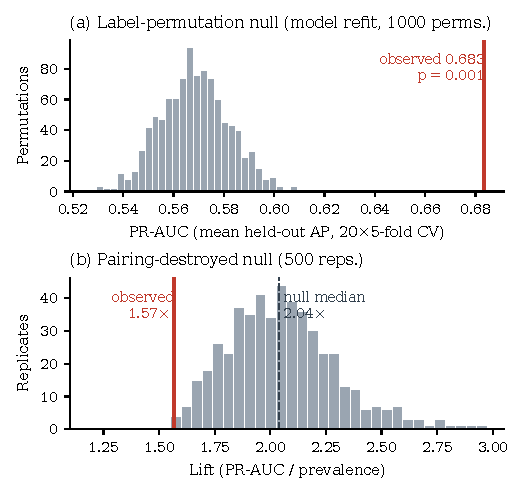
\includegraphics[width=\columnwidth]{figures/case1_nulls.pdf}
\caption{กรณีที่ 1 การออกแบบเดิม (a) เครื่องมือวินิจฉัยด้วยการสลับป้ายกำกับแบบเดิม
(สลับป้ายกำกับข้อมูลฝึกภายในแต่ละ Fold และฝึกแบบจำลองใหม่ ยังไม่ได้ตรวจการสอบเทียบ)
ซึ่งให้ค่า \textit{p} = 0.001 (b) Pairing-Destroyed Null ของ Lift
ที่คำนวณด้วยคะแนนอ้างอิง (มัธยฐาน 2.04 เท่า
หากฝึกแบบจำลองเต็มใหม่ทุกครั้งได้มัธยฐาน 1.99 เท่า) แบบจำลองไม่ผ่าน Null นี้
Null นี้เป็นแบบอนุรักษ์ การไม่ผ่านจึงหมายความเพียงว่ายังไม่มีหลักฐานของการตอบสนอง
ที่มากกว่าการถดถอยเข้าหาค่าเฉลี่ย ไม่ได้หมายความว่าไม่มีการตอบสนองนั้น}
\label{fig:case1}
\end{figure}

\subsection{ผลการจำลอง: ข้อมูลมากขึ้น การปฏิเสธยิ่งมั่นใจขึ้น}
\label{sec:simresults}
ผลการจำลองสองข้อทำให้ผู้วิจัยประหลาดใจมากกว่าข้อผิดพลาดเดิม (รูปที่~\ref{fig:sim})
ข้อแรก เมื่อไม่มีการตอบสนองที่พยากรณ์ได้และ \textit{r} = 0.25
การสลับป้ายกำกับของผลลัพธ์การเปลี่ยนแปลงดิบปฏิเสธสมมติฐานความเป็นอิสระ
ในร้อยละ 26 ของชุดข้อมูลเมื่อ \textit{n} = 50 และร้อยละ 100 เมื่อ \textit{n} = 500
การปฏิเสธแต่ละครั้งถูกต้องในเรื่องความเป็นอิสระ แต่ผิดหากใช้เป็นหลักฐานของการพยากรณ์
กลุ่มตัวอย่างที่ใหญ่ขึ้นช่วยประมาณความเชื่อมโยงได้แม่นยำขึ้น
แต่ไม่ได้ทำให้ความเชื่อมโยงหายไป ข้อสอง Residualisation รายสารบ่งชี้
ซึ่งถดถอยการเปลี่ยนแปลงของสารบ่งชี้แต่ละตัวบนค่าตั้งต้นของตัวเองเท่านั้น
และเป็นวิธีแก้ที่ใช้ในการวิเคราะห์ฉบับแก้ไขของผู้วิจัย
ยังปฏิเสธในร้อยละ 8--29 ของชุดข้อมูลจำลองที่ไม่มีการตอบสนองรายบุคคลที่พยากรณ์ได้ในเงื่อนไขต่าง ๆ
เพราะสารบ่งชี้ที่สัมพันธ์กันพาข้อมูลค่าตั้งต้นของกันและกันมาด้วย
Joint Residualisation ลดอัตรานี้เหลือร้อยละ 5--8
ซึ่งสูงกว่าระดับที่กำหนดไว้ร้อยละ 5 เล็กน้อย
วิธีแก้ไขก็เป็นการตรวจสอบอย่างหนึ่ง และต้องได้รับการตรวจสอบเช่นกัน

\begin{figure*}[t]
\centering
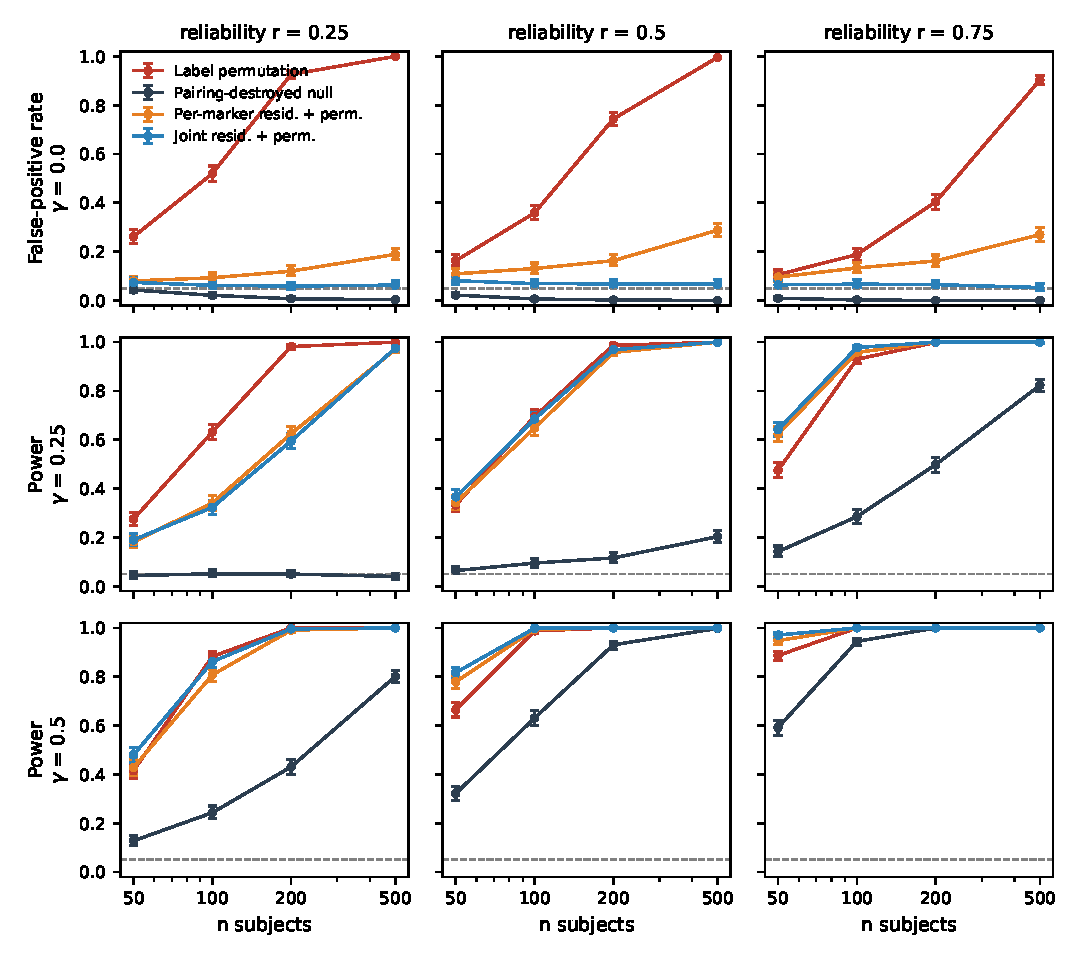
\includegraphics[width=0.8\textwidth]{figures/sim_rejection.pdf}
\caption{อัตราการปฏิเสธจากการจำลองเทียบกับจำนวนบุคคล (1,000 ชุดข้อมูลต่อจุด
แถบความคลาดเคลื่อนคือช่วงความเชื่อมั่น 95\% แบบ Wilson ของสัดส่วนการปฏิเสธ)
แถวแสดงขนาดของการตอบสนองที่พยากรณ์ได้ ($\gamma$ = 0, 0.25 และ 0.5)
คอลัมน์แสดงความเที่ยงของการวัด \textit{r} เมื่อ $\gamma$ = 0
ไม่มีการตอบสนองรายบุคคลที่พยากรณ์ได้ การปฏิเสธทุกครั้งในแถวบน
(แกนระบุว่า False-positive rate) จึงเป็นสัญญาณเท็จของความสามารถในการพยากรณ์
แม้จะปฏิเสธความเป็นอิสระได้ถูกต้องก็ตาม
สำหรับผลลัพธ์การเปลี่ยนแปลงดิบ การสลับป้ายกำกับทั้งชุดเพิ่มเข้าใกล้ร้อยละ 100
เมื่อ \textit{n} เพิ่มขึ้น Residualisation รายสารบ่งชี้ก็เพิ่มขึ้นเช่นกัน
ส่วน Joint Residualisation คงอยู่ที่ร้อยละ 5--8
แถวล่างแสดงอำนาจการทดสอบเมื่อมีการตอบสนองที่พยากรณ์ได้ เส้นประคือ $\alpha$ = 0.05}
\label{fig:sim}
\end{figure*}

\subsection{การทำซ้ำในกลุ่มตัวอย่างที่สอง}
ใน MTBLS881 เครื่องมือวินิจฉัยด้วยการสลับป้ายกำกับให้ค่า \textit{p} = 0.007
ที่ทั้งสองตำแหน่งสำหรับผลลัพธ์การเปลี่ยนแปลงดิบ
ทั้งสองตำแหน่งไม่แสดงว่าแบบจำลองดีกว่าคะแนนอ้างอิง
ช่วงความเชื่อมั่น 95\% ของผลต่างระหว่างแบบจำลองกับคะแนนนี้ครอบคลุมศูนย์ทั้งสองตำแหน่ง
(−0.037 [−0.231, +0.118] ที่ Left Atrium และ +0.013 [−0.111, +0.154]
ที่ Pulmonary Artery) ทั้งสองตำแหน่งมาจากผู้ป่วยกลุ่มเดียวกัน
จึงเป็นการสังเกตที่สัมพันธ์กัน ไม่ใช่การทำซ้ำสองครั้ง
และค่า \textit{p} มาจากวิธีสลับราย Fold แบบเดียวกันที่ยังไม่ได้ตรวจการสอบเทียบ
ในที่นี้ใช้กับแบบจำลองที่ไม่มีข้อจำกัด
ส่วนคำถามว่าหลัง Joint Residualisation ยังมีสัญญาณจริงเหลืออยู่หรือไม่
ผลจากผู้ป่วย 47 คนในชุดข้อมูลนี้ยังไม่ให้ข้อสรุปที่ชัดเจน

\subsection{กรณีที่ 2: คำอธิบายที่ซื่อตรงต่อสิ่งที่ผิด}
\label{sec:case2}

\storylabel{สิ่งที่ผู้วิจัยเชื่อ}ตัวจำแนกที่แยกตัวอย่างก่อนผ่าตัดกับเดือนที่ 12
(PR-AUC 0.973, CV แบ่งตามผู้ป่วย) พึ่งพาเมแทบอไลต์ที่บอกว่า
การผ่าตัดเปลี่ยนแปลงเมแทบอลิซึมอย่างไร และ ROAR ยืนยันว่าเป็นสารใดบ้าง

\storylabel{เหตุใดการตรวจสอบจึงผ่าน}การตัดฟีเจอร์ตามอันดับจาก SHAP ทีละตัวและฝึกใหม่
ทำให้แบบจำลองแย่ลงมากกว่าการตัดฟีเจอร์แบบสุ่มตั้งแต่การตัดครั้งที่สามเป็นต้นไป
ผลการตัดฟีเจอร์เชิงสำรวจนี้ชี้ว่าแบบจำลองพึ่งพาฟีเจอร์เหล่านั้น
แต่ฟีเจอร์ห้าตัวแรกที่ถูกตัดมี Dimethyl Sulfone, Isopropanol และ Methanol อยู่ด้วย
Isopropanol ใช้ทำความสะอาดผิวหนัง
และการจัดการระหว่างเก็บตัวอย่างอาจทำให้สารจากภายนอกปนเข้ามาในตัวอย่างได้
\cite{bernini2011, vandersar2015} แหล่งอ้างอิงเหล่านี้อธิบายความเสี่ยงทั่วไป
ไม่ได้ยืนยันการปนเปื้อนในข้อมูลกลุ่มนี้ ส่วน Dimethyl Sulfone เป็นเมแทบอไลต์ปกติในพลาสมา
ซึ่งมาจากอาหาร แบคทีเรียในลำไส้ และเมแทบอลิซึมของกำมะถันในร่างกาย \cite{engelke2005}
ซึ่งล้วนอาจต่างกันระหว่างก่อนและหลังผ่าตัด
ผู้วิจัยจึงถือว่าสารทั้งสามเป็นสารที่\textit{ยังไม่ทราบแหล่งที่มาแน่ชัด}
อาจสะท้อนชีววิทยา การจัดการตัวอย่าง หรือทั้งสองอย่าง
และการมาจากภายนอกร่างกายก็ไม่ได้หมายความว่าเป็นการปนเปื้อนระหว่างการจัดการตัวอย่างเสมอไป
ข้อมูลที่เผยแพร่ไม่สามารถตัดสินเรื่องนี้ได้ และข้อโต้แย้งต่อไปนี้ไม่ได้ขึ้นกับเรื่องนี้

\storylabel{สิ่งที่พบ}การตัดสารทั้งสามนี้ให้ PR-AUC 0.954
การตัดเมแทบอไลต์ที่เป็นที่ยอมรับสามชนิดให้ 0.959
การตัดทั้งสองแบบทำให้สมรรถนะต่ำกว่าการตัดแบบสุ่มเกือบทั้งหมด
ผลต่างที่สังเกตได้คือ 0.0056 เทียบกับส่วนเบี่ยงเบนมาตรฐานระหว่าง Fold ประมาณ 0.03
และผู้วิจัยไม่ได้ทำการทดสอบความเทียบเท่า (Equivalence Test) อย่างเป็นทางการ
กล่าวอีกนัยหนึ่ง ROAR ไม่ได้ส่งสัญญาณใดว่าสองกลุ่มนี้มีแหล่งที่มาต่างกัน
สำหรับฟีเจอร์ Artefact สังเคราะห์ที่มีขนาดผลใกล้เคียงกับ Dimethyl Sulfone
SHAP จัดให้เป็นอันดับหนึ่งใน 6 จาก 10 ครั้ง และอันดับสองในครั้งที่เหลือ
และค่ามัธยฐานของสมรรถนะที่ลดลงเมื่อตัดฟีเจอร์นี้เพียงตัวเดียวสูงกว่าเมแทบอไลต์จริงทุกตัว
ข้อควรระวังคือ การจัดอันดับด้วย SHAP คำนวณจากตัวอย่างทั้ง 177 ตัว
รวมถึงตัวอย่างที่ใช้ประเมินผลภายหลัง
การตัดฟีเจอร์ตามอันดับจึงมีความเอนเอียงจากการคัดเลือก (Selection Bias) ที่ไม่ทราบขนาด
\cite{varma2006} ผู้วิจัยจึงถือว่าการเปรียบเทียบ ROAR เป็นผลเชิงสำรวจ
และฟีเจอร์สังเคราะห์สนับสนุนประเด็นเชิงแนวคิดได้โดยไม่ต้องพึ่งการเปรียบเทียบเหล่านั้น

\storylabel{บทเรียน}การทดสอบความซื่อตรงของคำอธิบายต่อแบบจำลอง (Faithfulness Test)
ตรวจว่าฟีเจอร์ที่คำอธิบายให้ความสำคัญสอดคล้องกับฟีเจอร์ที่มีผลต่อการทำนายของแบบจำลองหรือไม่
ไม่ได้รับรองความถูกต้องของแบบจำลองโดยรวม การทดสอบแบบตัดฟีเจอร์
วัดว่าฟีเจอร์มีสัญญาณที่ไม่ซ้ำกับฟีเจอร์อื่นมากเพียงใด ไม่ว่าสัญญาณนั้นจะมาจากไหน
การทดสอบนี้ซื่อตรงต่อแบบจำลอง และแบบจำลองก็ซื่อตรงต่อสิ่งใดก็ตามที่แยกคลาสออกจากกัน
\cite{adebayo2018, kumar2020} ROAR จึงตัดสินแหล่งที่มาไม่ได้
ไม่สามารถบอกได้ว่าฟีเจอร์อันดับต้นสะท้อนชีววิทยา การจัดการตัวอย่าง หรือทั้งสองอย่าง
และสำหรับสารสามชนิดนี้ คำถามดังกล่าวยังคงเปิดอยู่

\subsection{กรณีที่ 3: ข้อมูลกลุ่มเดียวที่แท้จริงคือสองการศึกษา}
\label{sec:case3}

\storylabel{สิ่งที่ผู้วิจัยเชื่อ}สเปกตรัม NMR ของปัสสาวะแยกผู้ป่วยเบาหวานชนิดที่ 2
ออกจากกลุ่มควบคุมได้ด้วย PR-AUC 0.976 ภายใต้ CV ที่แบ่งตามบุคคล

\storylabel{เหตุใดการตรวจสอบจึงผ่าน}การแบ่งตามบุคคลป้องกันไม่ให้แบบจำลองจำบุคคลที่เคยเห็นแล้วได้
แต่ไม่สามารถตรวจพบความแตกต่างที่สมาชิกทุกคนในคลาสหนึ่งมีร่วมกัน

\storylabel{สิ่งที่พบ}ค่า 0.976 มาจาก Random Seed เดียว
เมื่อใช้ 20 Seed ค่าเฉลี่ยคือ 0.911 (ช่วง 0.845--0.975)
จากนั้นผู้วิจัยทำตารางไขว้ระหว่างป้ายกำกับกับคอลัมน์ Metadata ที่เผยแพร่ทั้ง 64 คอลัมน์
พบว่า 56 คอลัมน์มีค่าคงที่ และนอกจากรหัสประจำตัวอย่างแล้ว
มีเพียงเพศและป้ายกำกับที่มีค่าแปรผัน ไม่มีคอลัมน์ใดบันทึกวันที่ Batch หรือลำดับการวัด
อย่างไรก็ตาม โปรโตคอลที่เผยแพร่ระบุว่าข้อมูลมาจากสองการศึกษา
คือ อาสาสมัคร 12 คน อายุ 18--55 ปี เก็บตัวอย่าง 7 ช่วงเวลาที่กำหนด
และผู้ป่วยอายุ 30--65 ปีที่มีดัชนีมวลกายสูงกว่า เก็บตัวอย่าง 1--3 ครั้ง
ชื่อตัวอย่างของกลุ่มควบคุมทุกตัวขึ้นต้นด้วย \texttt{ADG19007u}
และของผู้ป่วยทุกตัวขึ้นต้นด้วย \texttt{ADG10003u}
การเป็นสมาชิกของกลุ่มการศึกษา รวมถึงตารางการเก็บตัวอย่าง
และความแตกต่างใด ๆ ในวิธีเก็บและเก็บรักษาปัสสาวะของสองการศึกษา
จึงปะปนกับป้ายกำกับอย่างสมบูรณ์ อายุและดัชนีมวลกายมีเกณฑ์คัดเข้าที่ต่างกันแต่ซ้อนทับกัน
จึงเป็นตัวแปรกวนที่เป็นไปได้ด้วย และไม่มีการบันทึกค่าเหล่านี้รายตัวอย่าง

ข้อจำกัดเชิงวิธีของการทบทวนครั้งนี้ควรกล่าวไว้ ณ ที่นี้
ข้อมูลว่าตัวอย่างใดเป็นของผู้ป่วยคนใดไม่ได้เผยแพร่
ผู้วิจัยจึงจัดกลุ่มตัวอย่างของผู้ป่วยด้วยวิธีอนุมานจากลำดับหมายเลข
ซึ่งรวมผู้ป่วยต่างคนกันอย่างน้อยสามคู่ไว้ในกลุ่มเดียวกัน
ซึ่งเป็นแบบอนุรักษ์สำหรับคู่เหล่านั้น
แต่ผู้วิจัยไม่สามารถตัดความเป็นไปได้ว่าวิธีนี้แยกตัวอย่างของผู้ป่วยคนเดียวกันไปอยู่คนละกลุ่ม
การจัดกลุ่มมีผลต่อคะแนนจริง ด้วย 20 Seed เดียวกัน CV ที่แบ่งตามบุคคลได้ 0.911
(0.906 เมื่อใช้การจัดกลุ่มอีกแบบที่สอดคล้องกับโปรโตคอล)
และ CV ที่ไม่แบ่งตามบุคคลได้ 0.969 อย่างไรก็ตาม ปัญหาโปรโตคอลไม่ได้ขึ้นกับการจัดกลุ่ม
เพราะเป็นคุณสมบัติของการออกแบบการศึกษา และไม่มีวิธีแบ่ง Fold ใดขจัดปัญหานี้ได้

\storylabel{บทเรียน}ตัวจำแนกอาจเรียนรู้โรคเบาหวาน โปรโตคอลการเก็บตัวอย่าง หรือทั้งสองอย่าง
ข้อมูลนี้ไม่สามารถบอกได้ว่าเป็นแบบใด เพราะแต่ละโปรโตคอลมีเพียงคลาสเดียว \cite{leek2010}
ข้อมูลชุดนี้ไม่สามารถแยกอิทธิพลของโรคออกจากอิทธิพลของโปรโตคอลการเก็บตัวอย่าง
จึงยังสรุปไม่ได้ว่าสมรรถนะของแบบจำลองสะท้อนความแตกต่างของโรคจริงหรือไม่

\subsection{กรณีที่ 4: ป้ายกำกับที่ถูกตั้งชื่อตามสิ่งอื่น}
\label{sec:case4}

\storylabel{สิ่งที่ผู้วิจัยเชื่อ}NMR ของซีรัมแยกคนอ้วนออกจากคนที่ไม่อ้วนได้ด้วย ROC-AUC 0.973
ซึ่งเป็น AUC ของเส้นโค้ง ROC เฉลี่ยจากการแบ่ง Stratified 5-Fold เพียงครั้งเดียว
(0.974 เมื่อรันซ้ำ)

\storylabel{เหตุใดการตรวจสอบจึงผ่าน}เมื่อทำการประเมินซ้ำ 10 ครั้งด้วยแบบจำลองเดิม
CV ที่แบ่งตามผู้ป่วยและที่ไม่แบ่งต่างได้ค่าเฉลี่ย ROC-AUC ราย Fold เท่ากับ 0.965
(เป็นตัวสรุปคนละแบบกับ AUC ของเส้นโค้งเฉลี่ย
การแบ่งที่รันซ้ำให้ค่าเฉลี่ย AUC ราย Fold เท่ากับ 0.976)
แม้ใน CV ที่ไม่แบ่งตามผู้ป่วย ร้อยละ 65 ของตัวอย่างทดสอบ
จะมีตัวอย่างอีกครั้งของผู้ป่วยคนเดียวกันอยู่ในข้อมูลฝึก
การกำจัดการรั่วไหลนี้ไม่ได้ทำให้คะแนนลดลง และความสอดคล้องนี้ดูน่าเชื่อถือ

\storylabel{สิ่งที่พบ}คลาส ``ไม่อ้วน'' คือการเก็บตัวอย่างเดือนที่ 12 หลังผ่าตัด
ของผู้ป่วยกลุ่มเดียวกัน จากผู้ป่วย 106 คน มี 71 คนที่อยู่ในทั้งสองคลาส
และมีตัวอย่างรวมกันร้อยละ 80 ของตัวอย่างทั้งหมด Metadata ไม่ได้บันทึกดัชนีมวลกาย
จึงไม่สามารถตรวจได้ว่าผู้ป่วยเดือนที่ 12 คนใดไม่อ้วนแล้ว
คะแนนนี้สะท้อนสิ่งใดก็ตามที่ต่างกันระหว่างคนคนหนึ่งก่อนผ่าตัดลดน้ำหนัก
กับคนเดิมหนึ่งปีต่อมา ทั้งน้ำหนักที่ลดลง และอาจรวมถึงอาหาร อาหารเสริม และยาหลังผ่าตัด
รวมทั้งระยะเวลาเก็บรักษาตัวอย่างที่ต่างกันหนึ่งปี
ข้อมูลนี้ไม่สามารถระบุได้ว่าคะแนนนี้มาจากภาวะอ้วน

\storylabel{บทเรียน}ชื่อที่ถูกต้องคือ ``การจำแนกก่อนและหลังการผ่าตัด''

\subsection{รูปแบบร่วมของทั้งสี่กรณี}
ในทุกกรณี การตรวจสอบชี้ว่าข้อมูลมีโครงสร้างที่ใช้พยากรณ์ได้
โดยมีข้อควรระวังเรื่องวิธีสลับป้ายกำกับและการเปรียบเทียบ ROAR เชิงสำรวจตามที่กล่าวไว้แล้ว
สิ่งที่การตรวจสอบยืนยันไม่ได้คือโครงสร้างนั้นมาจากไหน
ไม่ว่าจะมาจากการคำนวณผลลัพธ์ จากสารที่ยังไม่ทราบแหล่งที่มา
จากโปรโตคอลการเก็บตัวอย่าง หรือจากการผ่าตัด
คำอธิบายทางเลือกเหล่านี้ผ่านการตรวจสอบได้ง่ายพอ ๆ กับคำอธิบายทางชีววิทยาที่ผู้วิจัยคิดไว้
การผ่านการตรวจสอบจึงแยกคำอธิบายเหล่านี้ออกจากกันไม่ได้
มีนิสัยสามอย่างที่ทำให้มองข้ามปัญหานี้ได้ง่าย

\storylabel{รายงานการตรวจสอบ แต่ไม่รายงานคำอธิบายทางเลือก}ส่วนวิธีการวิจัยมักระบุการตรวจสอบที่ทำ
แต่แทบไม่ระบุคำอธิบายทางเลือกที่การตรวจสอบนั้นตั้งใจตรวจ
เมื่อระบุการตรวจสอบไว้แล้ว ผู้อ่านก็มักเข้าใจว่าเป็นใบรับรองความถูกต้องโดยรวม
ทั้งที่การตรวจสอบนั้นตรวจรูปแบบความล้มเหลวเพียงแบบเดียว

\storylabel{เชื่อตัวเลขที่ดูดีกว่า}ค่า \textit{p} ที่ต่ำกว่า ขนาดตัวอย่างที่ใหญ่กว่า
หรือ AUC ที่ใกล้ 1 ให้ความรู้สึกว่าเป็นหลักฐานที่หนักแน่นกว่า
กรณีที่ 1 และการจำลองแสดงสถานการณ์ที่ข้อมูลมากขึ้นทำให้การปฏิเสธมั่นใจขึ้น
แต่ไม่ได้ให้ข้อมูลมากขึ้น และกรณีที่ 3 แสดงคะแนนสูงที่ขึ้นกับ Seed
ซึ่งตั้งอยู่บนตัวแปรกวนจากการออกแบบการศึกษา ในกลุ่มตัวอย่างขนาดเล็ก
คะแนนที่ใกล้ 1 เป็นเหตุผลให้มองหาตัวแทน (Proxy) ไม่ใช่เหตุผลให้หยุดตรวจ

\storylabel{ตรวจแบบจำลอง แต่ไม่ตรวจป้ายกำกับ}การตรวจสอบทั้งหมดของผู้วิจัยถือว่าป้ายกำกับถูกต้องอยู่แล้ว
ความล้มเหลวสองในสี่กรณีอยู่ที่ตัวป้ายกำกับเอง (กรณีที่ 1 และ 4)
และอีกกรณีหนึ่ง (กรณีที่ 3) อยู่ที่วิธีเก็บตัวอย่างของแต่ละคลาส
การตรวจสอบแบบจำลองไม่ว่ามากเพียงใดก็เข้าไม่ถึงปัญหาที่อยู่ก่อนถึงแบบจำลอง

% ===========================================================================
\section{สรุปผลและแนวทางในอนาคต}
\label{sec:conclusion}

\subsection{สรุปผลการวิจัย}
งานวิเคราะห์ทั้งสี่งานของผู้วิจัยให้ผลที่ผู้วิจัยเคยถือว่าผ่านการตรวจสอบความถูกต้องแล้ว
แต่ในทุกงาน การตีความทางชีววิทยาที่ผู้วิจัยให้กับผลนั้นไม่มีหลักฐานรองรับหรือไม่สามารถระบุได้
แบบจำลองพยากรณ์ผู้ตอบสนองไม่แสดงหลักฐานว่าดีกว่าคะแนนอ้างอิงที่
\textit{n} = 71 ซึ่งเป็นการไม่มีหลักฐาน ไม่ใช่หลักฐานว่าพยากรณ์ไม่ได้
ผล ROAR เชิงสำรวจชี้ว่าแบบจำลองพึ่งพาฟีเจอร์ใด แต่ไม่ได้บอกว่าฟีเจอร์เหล่านั้นมาจากไหน
สำหรับตัวจำแนกเบาหวาน ข้อมูลนี้ไม่สามารถแยกได้ว่าสมรรถนะเกิดจากโรค
หรือจากโปรโตคอลการเก็บตัวอย่าง
และตัวจำแนกโรคอ้วนแท้จริงคือตัวจำแนกก่อนและหลังการผ่าตัด
การตรวจสอบที่ผ่านแสดงเพียงว่าได้ตรวจรูปแบบความล้มเหลวหนึ่งแบบ
ภายใต้สมมติฐานของการตรวจสอบนั้น ไม่ได้ยืนยันว่าการตีความถูกต้อง

ข้อสรุปเหล่านี้มีข้อจำกัด ผู้วิจัยทบทวนเฉพาะงานของตนเองบนข้อมูลสาธารณะขนาดเล็กสามชุด
ซึ่งเลือกมาเพราะสามารถตรวจสอบปัญหาได้จากไฟล์ที่เผยแพร่
และไม่ได้กล่าวอ้างว่าความล้มเหลวเหล่านี้พบบ่อยเพียงใดในงานวิจัยที่ตีพิมพ์
ข้อค้นพบเกี่ยวข้องกับแนวปฏิบัติในการตรวจสอบความถูกต้อง
และไม่ได้สนับสนุนหรือคัดค้านความรู้ทางชีววิทยาของโรคอ้วน การผ่าตัดลดน้ำหนัก หรือเบาหวาน
ผู้วิจัยไม่ได้แสดงว่าตัวจำแนกใดใช้\textit{เพียง} Artefact
แต่แสดงว่าการตรวจสอบไม่สามารถตัด Artefact ออกได้
แหล่งที่มาของสารสามชนิดในกรณีที่ 2 ยังไม่ได้รับการยืนยัน
ค่า \textit{p} ในกรณีที่ 1 และการทำซ้ำมาจากวิธีสลับราย Fold ที่ยังไม่ได้ตรวจการสอบเทียบ
การจำลองใช้ข้อมูลแบบเกาส์เซียน แบบจำลองเชิงเส้น และเกณฑ์ผลลัพธ์แบบเดียว
และ Joint Residualisation ที่การจำลองสนับสนุนก็ตัดความสัมพันธ์ที่แท้จริง
ระหว่างการเปลี่ยนแปลงกับค่าตั้งต้นออกด้วย
การตรวจสอบที่กล่าวถึงมีประโยชน์เมื่อใช้ให้ตรงกับสมมติฐานและเป้าหมาย
ประเด็นของบทความนี้คือ การผ่านการตรวจสอบเหล่านี้ยังไม่เพียงพอสำหรับการตีความทางชีววิทยา

\subsection{แนวทางในอนาคต}
สำหรับงานเมแทบอโลมิกส์ที่มีขนาดตัวอย่างเล็กในอนาคต รวมถึงงานของผู้วิจัยเอง
ผู้วิจัยเสนอให้ระบุคำอธิบายทางเลือกของคะแนนหลักก่อนเลือกการทดสอบ
และตั้งคำถามหกข้อต่อไปนี้ ซึ่งบทความคู่กันมีโค้ดอ้างอิงสำหรับแต่ละข้อ \cite{vyw}

\begin{enumerate}[label=\arabic*), leftmargin=*]
  \item \textit{ผลลัพธ์คำนวณจากฟีเจอร์หรือไม่} ถ้าใช่
        การสลับป้ายกำกับไม่ใช่หลักฐานของการพยากรณ์
        หากเป้าหมายคือการเปลี่ยนแปลงที่มากกว่าที่ค่าตั้งต้นทำนายไว้
        ให้ถดถอยการเปลี่ยนแปลงบนค่าตั้งต้น\textit{ทุกตัว}ภายในแต่ละ Fold ของข้อมูลฝึก
        แต่หากการเปลี่ยนแปลงที่ขึ้นกับค่าตั้งต้นเป็นสิ่งที่สนใจเอง วิธีนี้จะตัดสิ่งนั้นออก
        และคำถามนี้อาจต้องใช้การวัดค่าตั้งต้นซ้ำ
        หรือการออกแบบอื่นที่แยกความคลาดเคลื่อนของการวัดออกจากการตอบสนอง
        ไม่ว่ากรณีใด ให้รายงาน Pairing-Destroyed Null เป็นเครื่องมือวินิจฉัยทางเดียว
  \item \textit{ฝึกแบบจำลองใหม่ในทุกรอบของการสลับหรือไม่ และระบุวิธีสลับไว้หรือไม่}
        หากค่าสถิติที่สังเกตได้ต่ำกว่า Null ทั้งหมด ให้ตรวจวิธีสร้าง Null
        ขั้นตอนการให้คะแนน ข้อจำกัดของแบบจำลอง และวิธีฝึก ก่อนอ่านค่า \textit{p}
  \item \textit{แบบจำลองดีกว่าคะแนนอ้างอิงที่ไม่ต้องฝึกแบบจำลองหรือไม่}
        ให้รายงานผลต่างพร้อมช่วงความเชื่อมั่นที่สุ่มซ้ำระดับบุคคล
  \item \textit{มีฟีเจอร์ใดที่อาจมาจากการจัดการตัวอย่างหรือจากยาหรือไม่}
        ให้รายงานผลทั้งแบบมีและไม่มีฟีเจอร์เหล่านั้น
        และส่งฟีเจอร์ที่รู้แน่ว่าไม่มีความหมายทางชีววิทยาผ่านขั้นตอนการอธิบายฟีเจอร์
  \item \textit{มีคอลัมน์ Metadata หรือโปรโตคอลการเก็บตัวอย่างใดที่สอดคล้องกับป้ายกำกับหรือไม่}
        ให้ทำตารางไขว้ระหว่างป้ายกำกับกับทุกคอลัมน์ และอ่านว่าแต่ละคลาสเก็บตัวอย่างอย่างไร
  \item \textit{อะไรที่แยกสองคลาสออกจากกันในทางกายภาพ เมื่อเขียนเป็นประโยคเดียว}
        ถ้าประโยคนั้นต่างจากชื่อบทความ ให้เปลี่ยนชื่อบทความ
\end{enumerate}

คำถามเหล่านี้ใช้กับข้อมูลที่มีอยู่แล้วได้
แม้การแก้ปัญหาบางข้อที่พบอาจต้องใช้การวัดใหม่หรือการออกแบบการศึกษาที่ต่างออกไป
สำหรับการทบทวนครั้งนี้ มีการวิเคราะห์สี่อย่างที่จะช่วยเสริมหลักฐาน ได้แก่
การรันการทดสอบในกรณีที่ 1 สำหรับผลลัพธ์การเปลี่ยนแปลงดิบซ้ำด้วยการสลับป้ายกำกับทั้งชุด
เพื่อประเมินความไวของข้อสรุปต่อวิธีสลับป้ายกำกับ
การประเมินอัตราการปฏิเสธของวิธีสลับราย Fold จากข้อมูลจำลองซ้ำ
ภายใต้สมมติฐานว่างที่ต้องการทดสอบ เพื่อตรวจการสอบเทียบของวิธีนี้
(โดยแยกกรณีที่ไม่มีการตอบสนองที่พยากรณ์ได้ ออกจากกรณีที่ฟีเจอร์กับป้ายกำกับเป็นอิสระต่อกัน
ซึ่งไม่ใช่เงื่อนไขเดียวกัน)
การคำนวณอันดับ SHAP ของกรณีที่ 2 ภายในแต่ละ Fold ของข้อมูลฝึก
และการทำกรณีที่ 4 ซ้ำในข้อมูลที่มีการบันทึกดัชนีมวลกายและมีกลุ่มควบคุมที่ไม่อ้วน

% ===========================================================================
\section*{ข้อมูลและโค้ด}
ชุดข้อมูล MTBLS242, MTBLS1 และ MTBLS881 เผยแพร่สาธารณะผ่าน MetaboLights \cite{haug2020}
โค้ดการวิเคราะห์ การจำลอง และบันทึกตัวเลขทุกค่าที่รายงานพร้อมสคริปต์และ Random Seed
สามารถขอได้จากผู้วิจัย

\section*{กิตติกรรมประกาศ}
ผู้วิจัยขอขอบคุณที่ปรึกษาของงานวิจัยนี้
คือ ผศ.ดร.~นนท์~คนึงสุขเกษม แห่งคณะเทคโนโลยีสารสนเทศ
สถาบันเทคโนโลยีพระจอมเกล้าเจ้าคุณทหารลาดกระบัง
งานวิจัยนี้ไม่ได้รับทุนสนับสนุนเฉพาะ

% ===========================================================================
\renewcommand{\refname}{เอกสารอ้างอิง}
\begingroup
\small
\begin{thebibliography}{00}
\setlength{\itemsep}{0pt}\setlength{\parsep}{0pt}
\bibitem{vyw} Orrudee, C., \& Shomwiwat, K. C. (2026). \textit{Validated, yet wrong: Four ways small-n metabolomics machine learning passes standard checks} [Unpublished manuscript].
\bibitem{ojala2010} Ojala, M., \& Garriga, G. C. (2010). Permutation tests for studying classifier performance. \textit{Journal of Machine Learning Research, 11}, 1833--1863.
\bibitem{hooker2019} Hooker, S., Erhan, D., Kindermans, P.-J., \& Kim, B. (2019). A benchmark for interpretability methods in deep neural networks. \textit{Advances in Neural Information Processing Systems, 32}.
\bibitem{oldham1962} Oldham, P. D. (1962). A note on the analysis of repeated measurements of the same subjects. \textit{Journal of Chronic Diseases, 15}(10), 969--977. doi:10.1016/0021-9681(62)90116-9
\bibitem{barnett2005} Barnett, A. G., van der Pols, J. C., \& Dobson, A. J. (2005). Regression to the mean: What it is and how to deal with it. \textit{International Journal of Epidemiology, 34}(1), 215--220. doi:10.1093/ije/dyh299
\bibitem{tu2007} Tu, Y.-K., \& Gilthorpe, M. S. (2007). Revisiting the relation between change and initial value: A review and evaluation. \textit{Statistics in Medicine, 26}(2), 443--457. doi:10.1002/sim.2538
\bibitem{archie1981} Archie, J. P. (1981). Mathematic coupling of data: A common source of error. \textit{Annals of Surgery, 193}(3), 296--303. doi:10.1097/00000658-198103000-00008
\bibitem{leek2010} Leek, J. T., et al. (2010). Tackling the widespread and critical impact of batch effects in high-throughput data. \textit{Nature Reviews Genetics, 11}(10), 733--739. doi:10.1038/nrg2825
\bibitem{han2022} Han, W., \& Li, L. (2022). Evaluating and minimizing batch effects in metabolomics. \textit{Mass Spectrometry Reviews, 41}(3), 421--442. doi:10.1002/mas.21672
\bibitem{bernini2011} Bernini, P., Bertini, I., Luchinat, C., Nincheri, P., Staderini, S., \& Turano, P. (2011). Standard operating procedures for pre-analytical handling of blood and urine for metabolomic studies and biobanks. \textit{Journal of Biomolecular NMR, 49}(3--4), 231--243. doi:10.1007/s10858-011-9489-1
\bibitem{vandersar2015} van der Sar, S. A., et al. (2015). Ethanol contamination of cerebrospinal fluid during standardized sampling and its effect on \textsuperscript{1}H-NMR metabolomics. \textit{Analytical and Bioanalytical Chemistry, 407}(16), 4835--4839. doi:10.1007/s00216-015-8663-9
\bibitem{kapoor2023} Kapoor, S., \& Narayanan, A. (2023). Leakage and the reproducibility crisis in machine-learning-based science. \textit{Patterns, 4}(9), 100804. doi:10.1016/j.patter.2023.100804
\bibitem{collins2024} Collins, G. S., et al. (2024). TRIPOD+AI statement: Updated guidance for reporting clinical prediction models that use regression or machine learning methods. \textit{BMJ, 385}, e078378. doi:10.1136/bmj-2023-078378
\bibitem{haug2020} Haug, K., et al. (2020). MetaboLights: A resource evolving in response to the needs of its scientific community. \textit{Nucleic Acids Research, 48}(D1), D440--D444. doi:10.1093/nar/gkz1019
\bibitem{mtbls242} EMBL-EBI. (2017). \textit{MetaboLights study MTBLS242: Metabolomic fingerprint of severe obesity is dynamically affected by bariatric surgery in a procedure-dependent manner} [Data set]. สืบค้นจาก \url{https://www.ebi.ac.uk/metabolights/MTBLS242}
\bibitem{gralka2015} Gralka, E., Luchinat, C., Tenori, L., Ernst, B., Thurnheer, M., \& Schultes, B. (2015). Metabolomic fingerprint of severe obesity is dynamically affected by bariatric surgery in a procedure-dependent manner. \textit{The American Journal of Clinical Nutrition, 102}(6), 1313--1322. doi:10.3945/ajcn.115.110536
\bibitem{salek2007} Salek, R. M., et al. (2007). A metabolomic comparison of urinary changes in type 2 diabetes in mouse, rat, and human. \textit{Physiological Genomics, 29}(2), 99--108. doi:10.1152/physiolgenomics.00194.2006
\bibitem{maltesen2020} Maltesen, R. G., Wimmer, R., \& Rasmussen, B. S. (2020). A longitudinal serum NMR-based metabolomics dataset of ischemia-reperfusion injury in adult cardiac surgery. \textit{Scientific Data, 7}, 198. doi:10.1038/s41597-020-0545-0
\bibitem{engelke2005} Engelke, U. F. H., Tangerman, A., Willemsen, M. A. A. P., Moskau, D., Loss, S., Mudd, S. H., \& Wevers, R. A. (2005). Dimethyl sulfone in human cerebrospinal fluid and blood plasma confirmed by one-dimensional \textsuperscript{1}H and two-dimensional \textsuperscript{1}H--\textsuperscript{13}C NMR. \textit{NMR in Biomedicine, 18}(5), 331--336. doi:10.1002/nbm.966
\bibitem{varma2006} Varma, S., \& Simon, R. (2006). Bias in error estimation when using cross-validation for model selection. \textit{BMC Bioinformatics, 7}, 91. doi:10.1186/1471-2105-7-91
\bibitem{adebayo2018} Adebayo, J., Gilmer, J., Muelly, M., Goodfellow, I., Hardt, M., \& Kim, B. (2018). Sanity checks for saliency maps. \textit{Advances in Neural Information Processing Systems, 31}.
\bibitem{kumar2020} Kumar, I. E., Venkatasubramanian, S., Scheidegger, C., \& Friedler, S. (2020). Problems with Shapley-value-based explanations as feature importance measures. \textit{Proceedings of the 37th International Conference on Machine Learning (ICML)}, PMLR 119, 5491--5500.
\end{thebibliography}
\endgroup

\end{document}
